%{{{ Formatierung

\documentclass[a4paper,12pt]{article}

\usepackage{physics_notetaking}

%%% dark red
%\definecolor{bg}{RGB}{60,47,47}
%\definecolor{fg}{RGB}{255,244,230}
%%% space grey
%\definecolor{bg}{RGB}{46,52,64}
%\definecolor{fg}{RGB}{216,222,233}
%%% purple
%\definecolor{bg}{RGB}{69,0,128}
%\definecolor{fg}{RGB}{237,237,222}
%\pagecolor{bg}
%\color{fg}

\newcommand{\td}{\,\text{d}}
\newcommand{\RN}[1]{\uppercase\expandafter{\romannumeral#1}}
\newcommand{\zz}{\mathrm{Z\kern-.3em\raise-0.5ex\hbox{Z} }}
\newcommand{\id}{1\kern-.258em1}

\newcommand\inlineeqno{\stepcounter{equation}\ {(\theequation)}}
\newcommand\inlineeqnoa{(\theequation.\text{a})}
\newcommand\inlineeqnob{(\theequation.\text{b})}
\newcommand\inlineeqnoc{(\theequation.\text{c})}

\newcommand\inlineeqnowo{\stepcounter{equation}\ {(\theequation)}}
\newcommand\inlineeqnowoa{\theequation.\text{a}}
\newcommand\inlineeqnowob{\theequation.\text{b}}
\newcommand\inlineeqnowoc{\theequation.\text{c}}

\renewcommand{\refname}{Source}
\renewcommand{\sfdefault}{phv}
%\renewcommand*\contentsname{Contents}

\pagestyle{fancy}

\sloppy

\numberwithin{equation}{section}

%}}}

\begin{document}

%{{{ Titelseite

\title{1 $|$ Ausbreitung von Signalen auf Leitungen}
\author{Angelo Brade, Jonas Wortmann}
\maketitle
\pagenumbering{gobble}

%}}}

\newpage

%{{{ Inhaltsverzeichnis

\fancyhead[L]{\thepage}
\fancyfoot[C]{}
\pagenumbering{arabic}

\tableofcontents

%}}}

\newpage

%{{{

\fancyhead[R]{\leftmark\\\rightmark}

\section{Einleitung}
In diesem Versuch werden Koaxialkabel behandelt und ihre Eigenschaften behandelt.
Die Reflexionseigenschaften innerhalb von Koaxialkablen sollen verstanden, sowie die Verzögerungszeit eines Kabels gemessen werden.
Zudem soll das Rechtecksignal eines Hochpasses differenziert werden.

\newpage
\section{Theorie}
Eine Doppelleitung (Hin-- und Rückleiter), deren elektrische Eigenschaften längs der ganzen Strecke gleichbleiben, nennt man homogene Leitung.
Koaxialkabel sind homogene Leitungen und bestehen aus einem leitenden Draht in der Mitte, darum ein Dielektrikum und wieder darum ein Geflecht aus einem leitenden Material welches Strahlung abschirmt.
Das ganze Kabel ist isoliert.
\\\indent Kabel können auch näherungsweise über eine Kette von LC--Gliedern dargestellt werden.
Hier verteilt sich die gesamte Induktivität und Kapazität über das gesamte Kabel.
Ein Ersatzschaltbild für die Wellenausbreitung in einem Leiter ist
\begin{figure}[h]
        \centering
        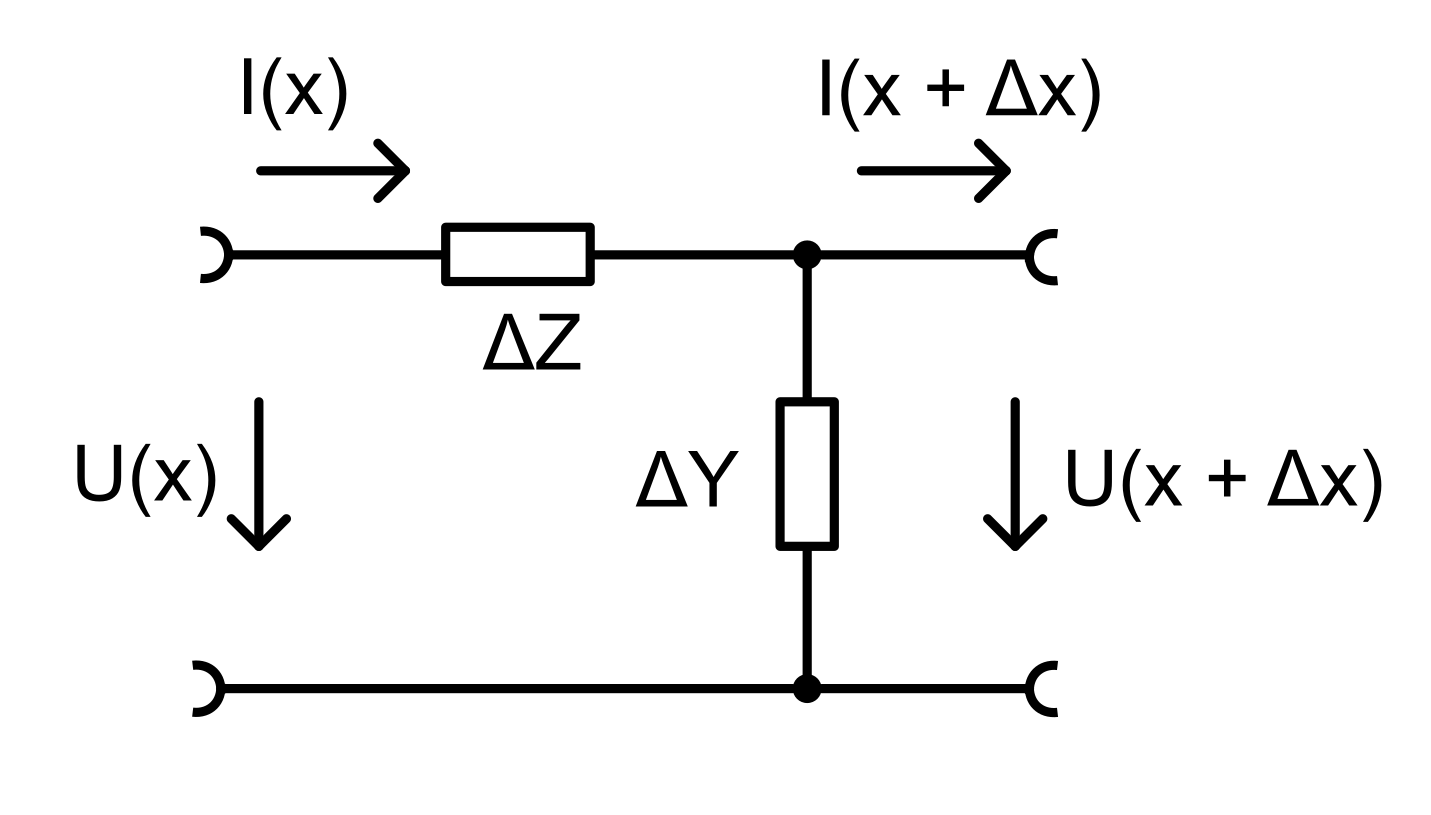
\includegraphics[width=0.8\textwidth]{ersatz_wellenausbreitung.png}
        \caption{Ersatzschaltbild zur Wellenausbreitung; Abbildung 1.3 \cite{Praktikumsanleitung}}
\end{figure}
Der Wellenwiderstand eines Kabels ist definiert als 
\begin{align} 
        Z=\dfrac{U_h\left(x\right)}{I_h\left(x\right)}=\dfrac{U_r\left(x\right)}{-I_r\left(x\right)}
,\end{align} 
mit $_h$ der Hinrichtung und $_r$ der Rückrichtung.
Im verlustfreien Fall ist $Z=\,\sqrt[]{\tfrac{L'}{C'}}$, also rein reell.
Für ein Koaxialkabel mit Innenradius $R_i$ und Außenradius $R_a$ gilt
\begin{align} 
        Z=Z_\text{frei}\cdot \dfrac{\ln\left(\tfrac{R_a}{R_i}\right)}{2\pi }
,\end{align} 
wobei $Z_\text{frei}=\,\sqrt[]{\tfrac{\mu _0}{\varepsilon _0}}=120\pi \,\SI{}{\ohm}$ der Wellenwiderstand des Vakuums ist.
\\\indent Es existieren drei verschiedene wichtige Möglichkeiten für den Abschlusswiderstand in einer Leitung.
\begin{enumerate}[label=--]
        \item Angepasster Abschluss: $R_A=Z,r=0,s=1,m=1$ 
        \item Offene Leitung: $R_A=\infty,r=+1,s=\infty,m=0$ 
        \item Kurzschluss: $R_A=0,r=-1,s=\infty,m=0$ 
\end{enumerate}
Hier beschreiben $R_A$ den Abschlusswiderstand, $r$ den Reflexionskoeffizienten, $s$ das Stehwellenverhältnis und $m$ den Anpassungsfaktor.

\newpage
\section{Voraufgaben}
\subsection{A}
Um große Verzögerungszeiten zu erreichen muss eine kleine Phasengeschwindigkeit sichergestellt werden, entsprechend große Permeabilität und Permitivität.

\subsection{B}
Wird die Verzögerungszeit über die Phasengeschwindigkeit geändert, so ändert sich auch der Wellenwiderstand, da diese Größen verschiedene Proportionalitäten besitzen
\begin{align} 
        v_{\text{ph}}\propto \dfrac{1}{\,\sqrt[]{L'C'}}\qquad Z\propto \,\sqrt[]{\dfrac{L'}{C'}}
.\end{align} 
Das Aufwickeln des Innenleiters um einen Ferritkern damit die Induktivität des Kabels gesteigert wird ändert den Wellenwiderstand nicht.

\subsection{C}
Sei ein Kabel abgeschlossen mit $R_A=Z$, findet keine Reflexion statt.
Alle Energie, die am Eingang des Kabels einläuft, wird am Kabelende vollständig an den Verbraucher $R_A$ abgegeben, da dieser wie eine Fortsetzung des Kabels aussieht.
Der Eingangswiderstand ist hier also unabhängig von der Länge des Kabels.

\subsection{D WIP Z}
Sei ein verlustfreier idealer Leiter mit den Eigenschaften $\tfrac{R_A}{R_I}=2.3,\varepsilon _r=1.5$ und $\mu _r=1.5$.
Dann ist die Phasengeschwindigkeit
\begin{align} 
        v_{\text{ph}}&=\dfrac{c_0}{\,\sqrt[]{\varepsilon _r\mu _r}}=\dfrac{c_0}{1.5}\approx \SI{1.93e+8}{m.s ^{-1}}
,\end{align} 
der Wellenwiderstand
\begin{align} 
        Z=
\end{align} 
und die Verzögerung
\begin{align} 
        \Delta =\dfrac{1}{v_{\text{ph} }}=\dfrac{1.5}{c_0}\approx \SI{5.2e-9}{s.m ^{-1}}\approx \SI{5.2}{\nano s.m ^{-1}}
.\end{align} 


\newpage
\section{Auswertung}

\clearpage
\listoffigures
\listoftables
\bibliographystyle{plain}
\bibliography{refs}

%}}}

\end{document}
